\documentclass[fontsize=10.5, ngerman]{scrreport}
\usepackage{stylefile}
\usepackage{svg}
\begin{document}
	
	\begin{titlepage}
		\centering
		\vspace*{\fill}
		\begin{center}
			\rule[0.5ex]{.8\textwidth}{2pt}\\
			\LARGE Optimierung der Feldeinstellungen in\\
			einem Triple- GEM-Detektor\\
			\rule[0.5ex]{.8\textwidth}{2pt}\\
			\vspace{0.5 cm}
			\large Bachelorarbeit in Physik\\
			\vspace{0.5 cm}
			von \\
			\vspace{0.5 cm}
			Maximilian Thomas Spors\\
			\vspace{0.5 cm}
			angefertigt am \\
			\vspace{0.5 cm}
			Helmholtz Institut für Strahlen und Kernphysik\\
			\vspace{1 cm}
			vorgelegt an der \\
			Mathematisch-Naturwissenschaftlichen Fakultät\\
			der Universität Bonn\\
			\vspace{1 cm}
			09/2024		
		\end{center}
		
		\vspace*{\fill}
	\end{titlepage}
	\newpage
	\pagenumbering{roman}
	\pagestyle{empty}
	\vspace*{\fill}
	\noindent	Ich versichere, dass ich diese Arbeit selbstständig verfasst und keine anderen als die angegebenen
	Quellen und Hilfsmittel benutzt sowie die Zitate kenntlich gemacht habe.
	
	
	\vspace{1.5 cm}
	
	
	\noindent \begin{minipage}[c]{6cm}
		Bonn, der\centering \dotfill
	\end{minipage} \hfill 
	\begin{minipage}[c]{6cm}
		Unterschrift: \centering \dotfill
	\end{minipage}
	
	\vspace{2cm}
	
	\noindent 1. Gutachter: Prof. Dr. Bernhard Ketzer\\
	\noindent 2. Gutachter:
	\newpage
	\pagestyle{scrheadings}
	\tableofcontents
	\newpage
	
	\pagenumbering{arabic}
	
	\chapter{Einleitung}


\noindent Das Standardmodell der Elementarteilchen beschreibt die fundamentalen Teilchen und Kräfte, die das Universum bestimmen. Seine Weiterentwicklung und Verfeinerung beruhen wesentlich auf dem genaueren Verständnis der Teilchen und ihrer Wechselwirkungen, die über Detektoren beobachtbar sind.\\
\\
Moderne Detektoren lassen sich in Klassen einteilen, die sich in ihren Anwendungen erheblich unterscheiden: Szintillationsdetektoren wandeln die Energie der eintreffenden ionisierenden Strahlung in Lichtpulse um, deren Messung sowohl eine genaue Bestimmung der im Detektor deponierten Energie als auch eine präzise zeitliche Zuordnung der Detektionsereignisse ermöglicht.\\
Halbleiterdetektoren wandeln die ionisierende Strahlung in Elektronen-Loch-Paare um, die zu messbaren Signalen führen. Da Halbleiter dichte Medien mit vergleichsweise geringer Ionisationsenergie sind, erlauben sie eine präzise Bestimmung der im Detektor deponierten Energie.\\
Gasdetektoren nutzen ähnliche physikalische Grundprinzipen, wobei hierbei Elektronen-Ionen-Paare erzeugt werden. Aufgrund ihrer geringeren Dichte und der Höheren Ionisationsenergie im Vergleich zu Halbleitern, ist die Energieauflösung etwas geringer. Dennoch haben sich Gasdetektoren durch ihre einfache Handhabung und Empfindlichkeit in vielen Anwendungen etabliert.  \cite{Leo}.\\
\\
Gasdetektoren sind besonders relevant, da sie in experimentellen Anordnungen aufgrund ihrer Robustheit und Flexibilität verwendet werden. Mit wachsenden Anforderungen, die für Experimente mit größerer Ereignisrate an die Detektoren gestellt werden, müssen dabei innovative Detektorkonzepte erdacht und Bestehende optimiert werden. In diese Entwicklung gliedert sich die Konzeption der Gas Electron Multiplier ein, die die Unzulänglichkeiten der zu diesem Zeitpunkt vorherrschenden Multiwire Proportional Chambers (MWPC) \cite{Sauli_Multiwire} \cite{GEM_Introduction} in Teilen kompensieren sollte. \\
Nach der Etablierung der Gas Electrom Multiplier setzte ein Optimierungsprozess ein, der sich bisher auf extensive Untersuchungen zur Detektorgeometrie \cite{BUTTNER},\cite{Bachmann}, auf die Wahl des aktiven Mediums \cite{GAS_MIX} und auf die Verbesserung der Stabilität der Detektorkonfiguration im Hinblick auf Gasentladungen \cite{Stabilitaet_Discharge} beschränkt, erste Untersuchungen für die Einstellungen  der Feldkonfiguration wurden bereits angestellt \cite{Bachmann},\cite{ottnad}, eine extensive experimentelle Untersuchung, Analyse und Optimierung der Feldeinstellungen steht dennoch aus. An diesem Punkt setzt diese Arbeit an.\\
\\
In dieser Arbeit soll die Wirkung der elektrischen Felder, die zum Betrieb des Gas Electron Multiplier verwendet werden, auf die Energieauflösung und die Signalverstärkung untersucht werden. Auf Basis dieser Ergebnisse, sollen dann Detektorkonfigurationen bestimmt werden, die es ermöglichen eine ähnliche, wenn nicht bessere Performance des Detektors bei geringerem Aufwand zu ermöglichen.\\
\\
Zu diesem Zweck wird in Kapitel II die grundlegende Funktionsweise von Gasdetektoren erörtert, wobei diese auf die zugrundeliegenden physikalischen Prinzipien reduziert werden. Damit kann dann die Spezielle Geometrie und Funktionsweise der Gas Electron Multiplier in Kapitel III skizziert werden, sodass in den Kapiteln IV und V die Wirkung des Feldes auf die Verstärkung und die Energieauflösung verstanden werden kann. Mit den Ergebnissen aus diesen Analysen lassen sich dann in Kapitel VI verschiedene interessante Detektorkonfigurationen bestimmen, die für weitere Analysen interessant sind. 

	\newpage
	\chapter{Funktionsweise von Gasdetektoren}

\noindent Gasgefüllte Detektoren sind eine effiziente Methode zur Untersuchung ionisierender Strahlung und physikalischer Wechselwirkungen, die zu Teilchenzerfällen führen. Das Verständnis ihrer Funktionsweise und inhärenten Grenzen erfordert die Diskussion der ihnen zugrundeliegenden physikalischen Mechanismen. In diesem Kapitel wird daher die Funktionsweise von Gasdetektoren auf Basis dieser Prinzipien erläutert.

	\section{Wechselwirkungen von ionisierender Strahlung mit Materie}
	Ionisierende Strahlung interagiert mit dem durchstrahlten Medium und kann dabei Ionisationen verursachen.  Die Wechselwirkungen unterscheiden sich für Photonen und geladenen Teilchen: Geladene Teilchen deponieren den Großteil ihrer Energie durch inelastische Stöße mit den Elektronen des Materials \cite{Leo}. Dieser Prozess hinterlässt eine Spur von Elektron-Ionen-Paaren im Material, was prinzipiell eine Rekonstruktion der Teilchenspur ermöglicht, und so beispielsweise die Analyse von Zerfallsprozessen erlaubt.\\
	\\
	Da die Spurrekonstruktion in dieser Arbeit keine zentrale Rolle spielt, werden im Folgenden nur die relevanten, nämlich die photonischen Wechselwirkungsphänomene fokussiert behandelt. Eine umfassende und detaillierte Behandlung der Teilchenwechselwirkungen findet sich exemplarisch in \cite{Leo} und \cite{Sauli_Multiwire}.

	\subsection{Photonen in Materie} \label{chap:Photonen}
	Die Wechselwirkung von Photonen mit Materie erfolgt im Wesentlichen durch den photoelektrischen Effekt, die Compton-Streuung und die Paarbildung.  Die Wahrscheinlichkeit dieser Prozesse hängt vom Material und der Photonenenergie $E_{\gamma}$ ab. Abbildung \ref{fig:WirkungsquerschnittePhotonen} veranschaulicht diesen Zusammenhang, indem sie die Bereiche darstellt, in denen die einzelnen Prozesse in Abhängigkeit von der Kernladungszahl und der Photonenenergie dominieren. Im Folgenden werden diese Prozesse kurz erläutert:
	\begin{figure}[h]
		\centering
		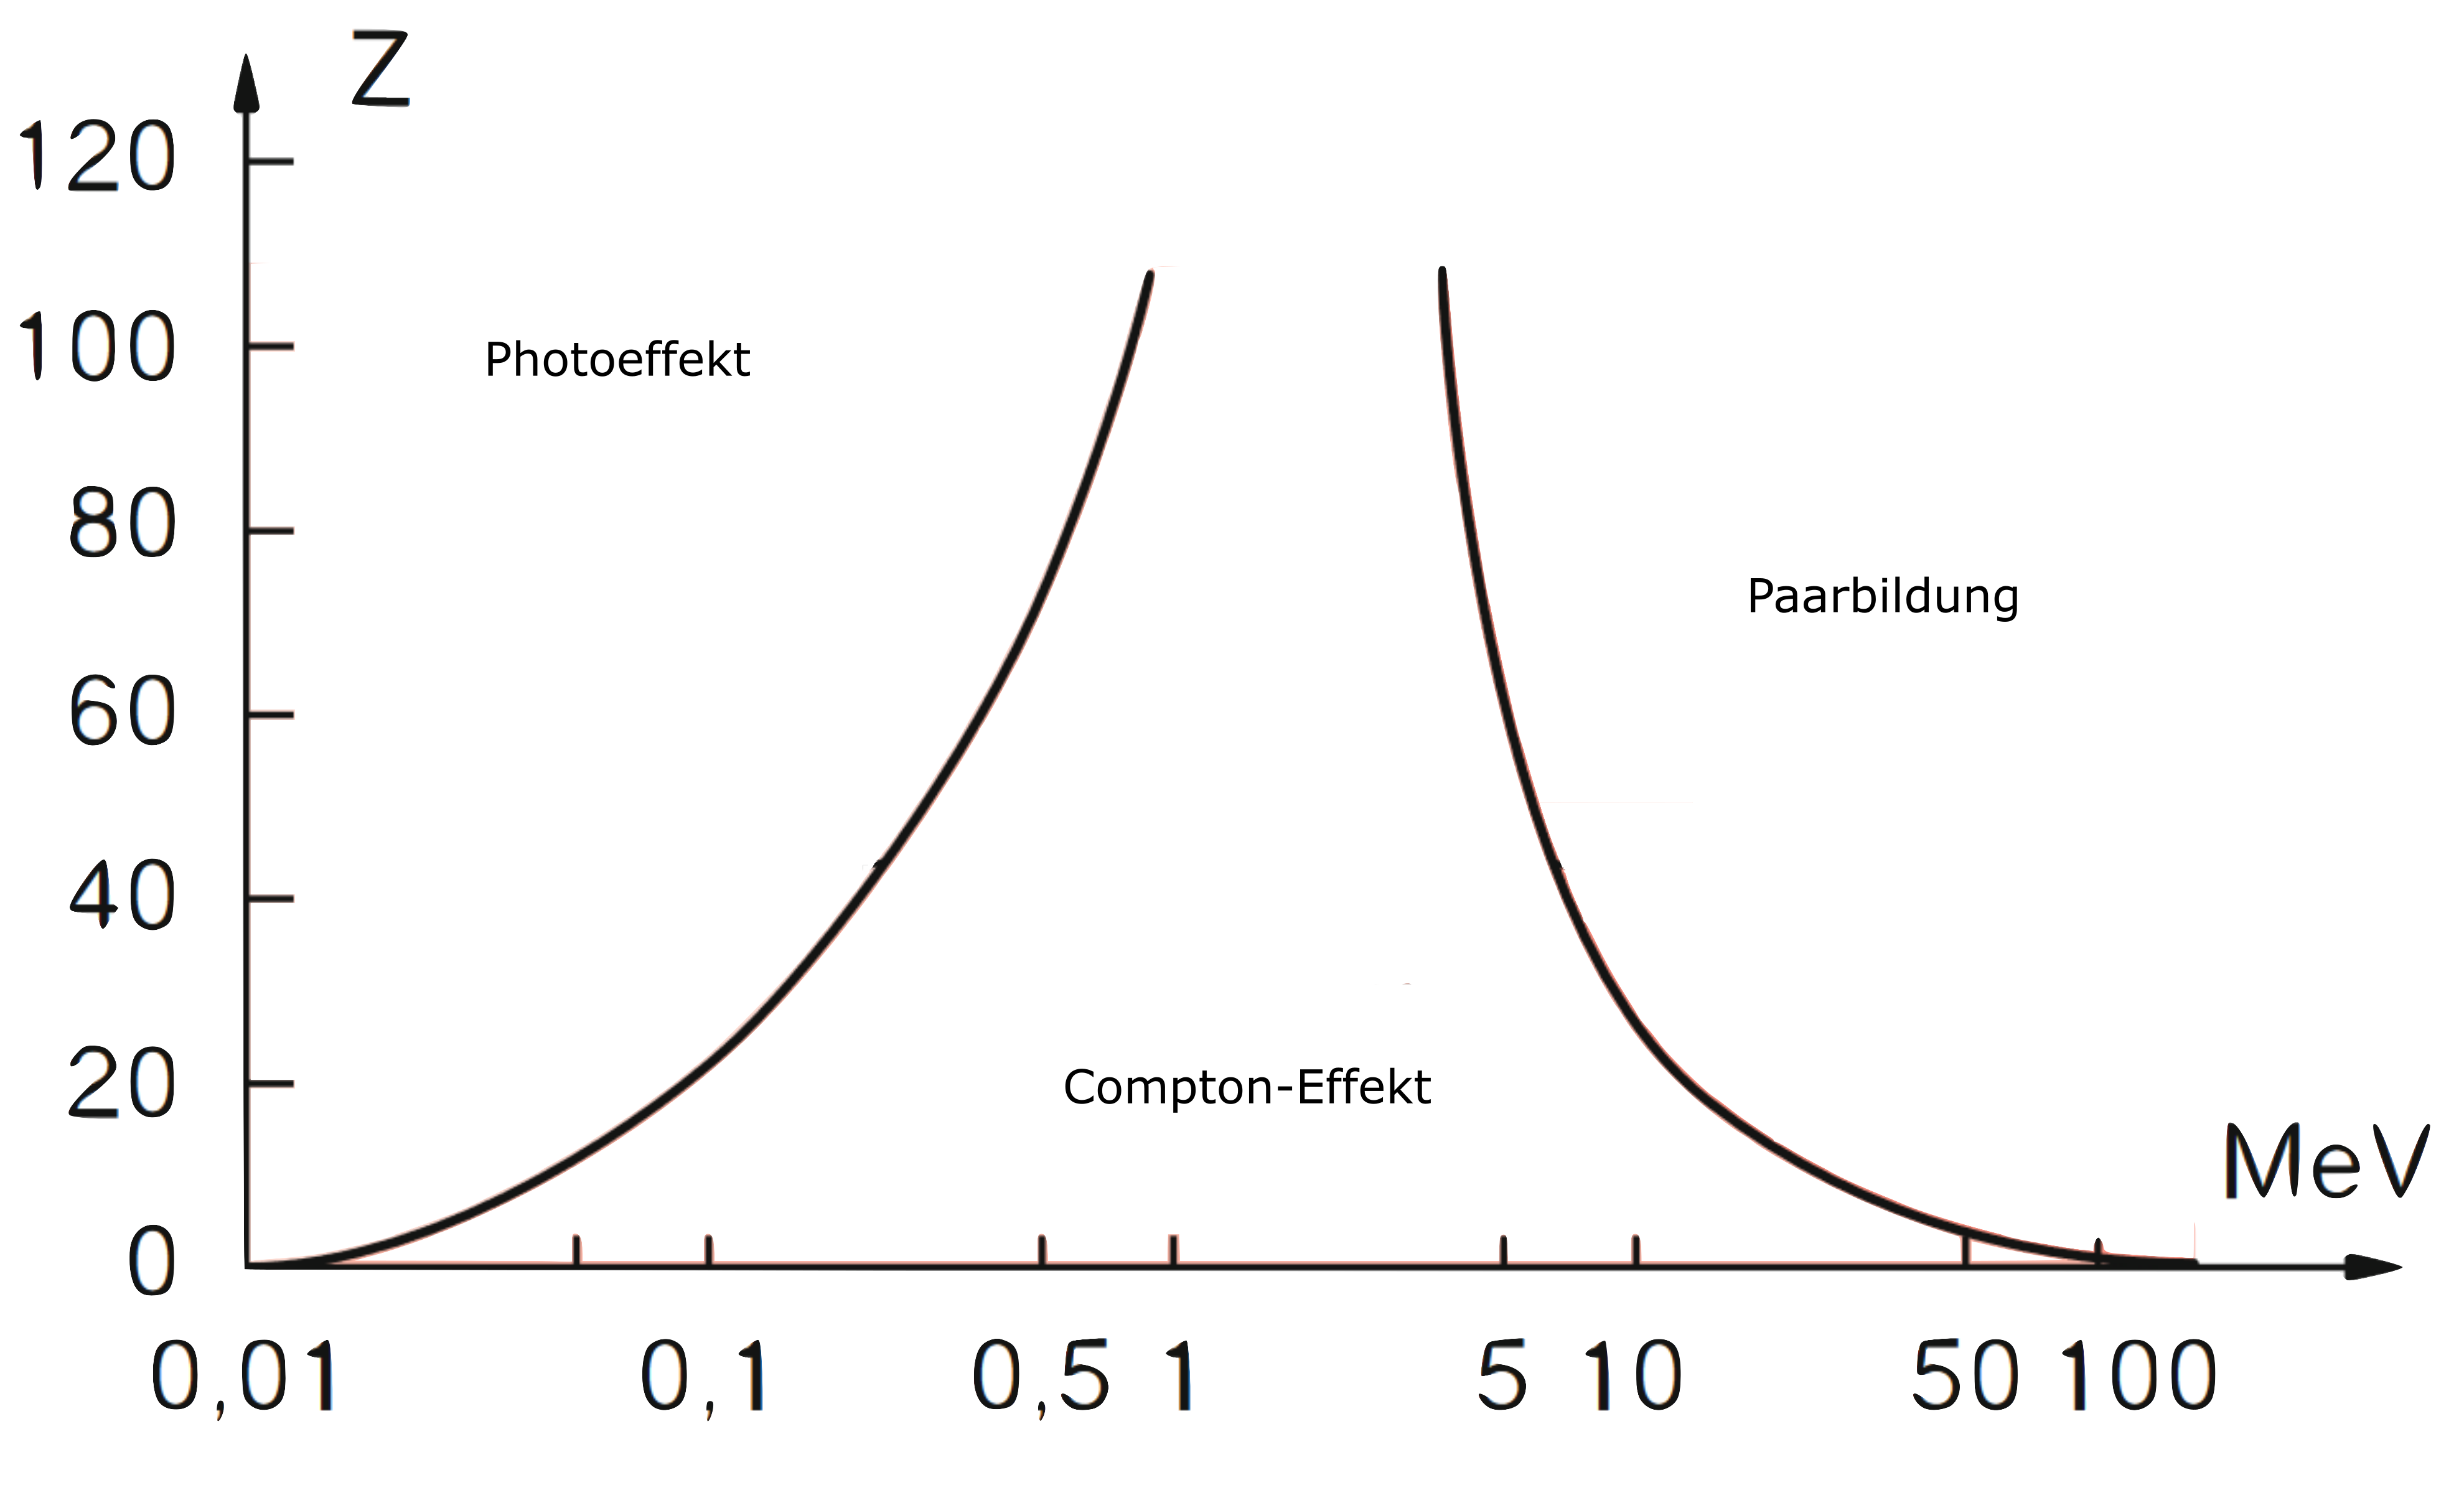
\includegraphics[scale=0.25]{PhotoQuerschnitte.png}
		\caption{Dominante Wechselwirkungen von Photonen in Abhängigkeit von der Kernladungszahl $Z$ des Absorbermaterials und der Photonenenergie. Die durchgezogenen Linien markieren die Grenzbereiche der dominierenden Effekte (modifiziert nach \cite{DemtroderKerne})}
		\label{fig:WirkungsquerschnittePhotonen}
	\end{figure}
	
		\subsubsection{Photoelektrischer Effekt}
		Der photoelektrische Effekt beschreibt die Absorption eines Photons durch ein gebundenes Elektron, wodurch das Atom angeregt oder ionisiert wird. Dieser Effekt dominiert im niederenergetischen Bereich (siehe Abbildung \ref{fig:WirkungsquerschnittePhotonen}). Mit der Bindungsenergie $\phi_{\text{A}}$ des Elektrons gilt für die Energie des auslösten Elektrons:
		\begin{equation*}
			E_{e^{-}}= E_{\gamma}-\phi_{\text{A}}
		\end{equation*} 
		
		\noindent Der Wirkungsquerschnitt ist sowohl kernladungszahl- als auch energieabhängig, wobei der folgende Zusammenhang gilt:
		\begin{equation*}
			\sigma= \frac{32\sqrt{2}}{3} \pi r_{\text{e}}^{2} \alpha^{4} Z^{5} \qty(\frac{m_{e}c^{2}}{h \nu})^{7/2}
		\end{equation*}
		Hierbei bezeichnet $Z$ die Kernladung des Atoms, $r_{\text{e}}$ den klassischen Elektronenradius, $\alpha\approx 1/137$ die Feinstrukturkonstante, $m_{e}$ die Elektronenruhemasse, $c$ die Lichtgeschwindigkeit, $h$ das Planck'sche Wirkungsquantum und $\nu$ die Frequenz der einfallenden Strahlung. Der Wirkungsquerschnitt steigt stark an, wenn die Strahlungsenergie geringfügig über den Ionisationsenergien der K-, L- und M-Schalen liegt und muss in diesen Bereichen durch Vorfaktoren korrigiert werden \cite{Leo}.

		
		
		\subsubsection{Compton-Streuung}
		Compton-Streuung ist die Streuung eines Photons an einem lose gebundenen Elektron. Ein Teil der Photonenenergie wird dabei auf das Elektron übertragen, das Photon wird nicht absorbiert. Man unterscheidet zwischen Rayleigh-, Thomson- und Compton-Streuung. Diese Phänomene werden durch die Klein-Nishina-Formel beschrieben, wobei die klassische Streuung den niederenergetischen Grenzfall der Compton-Streuung darstellt. Der Wirkungsquerschnitt der Compton-Streuung ist primär energieabhängig mit $\kappa=h\nu /(m_{e}c^{2})$ gilt  \cite{Leo}:
		\begin{equation*}
			\sigma= 2\pi r_{e}^{2} \qty(\frac{1+\kappa}{\kappa^{2}} \qty(\frac{2(1+\kappa)}{1+2\kappa}-\frac{\ln(1+2\kappa)}{\kappa})+\frac{\ln(1+2\kappa)}{2\kappa}-\frac{1+3\kappa}{(1+2\kappa^{2})})
		\end{equation*}
		
		
		
		\subsubsection{Paarbildung}
		Photonen deren Energie einen Wert von $1,22\ \si{MeV}$ überschreiten, können sich im Feld eines Kerns zu Elektronen-Positronen-Paaren umwandeln. Eine Umwandlung ohne einen dritten Wechselwirkungspartner ist aufgrund der Impulserhaltung nicht möglich. Paarbildung wird damit nur für hochenergetische Strahlung relevant. Der Wirkungsquerschnitt skaliert mit \cite{DemtroderKerne}:
		\begin{equation*}
			\sigma \propto Z^{2}\ln(E_{\gamma})
		\end{equation*} 
		
		
	\newpage
	
	\subsection{Sekundärionisation}	\label{chap:Sekundär}
		Nach der Primärionisation durch das Detektionsereignis gibt es Effekte, die Sekundärionisationen herbeiführen. In diesem Abschnitt sollen diese Erscheinungen diskutiert werden. 
		
		\subsubsection{Lokale Clusterbildung}
			Ein durch Strahlung erzeugtes freies Elektron hat oft noch so viel Energie, dass weitere Stoßwechselwirkungen mit den Atomen zu Sekundärionisationen führen. Es bildet sich ein lokales Cluster aus Elektronen, die zu einem Ereignis gehören, da der Ionisationsprozess so lange geht, bis die Energie des Elektrons für weitere Ionisationen nicht mehr ausreicht. Bei bekannter Ionisationsenergie des Mediums kann die Zahl der durch ein Detektionsereignis erzeugten Elektronen-Ionen-Paare kann wie folgt approximiert werden \cite{Sauli_Multiwire}:
			\begin{equation} \label{eq:Primärionisation}
				N_{\text{e}}=\frac{E_{\gamma}}{\phi_{\text{ion}}}
			\end{equation}	
			Hierbei handelt es sich um einen Erwartungswert, da die Zahl der erzeugten Paare aufgrund der statistischen Natur der Wechselwirkungen gemäß einer Polya-Verteilung fluktuiert. \cite{ottnad}.
		
		\subsubsection{Penning-Effekt}
			Durch die Beimischung eines Quencher-Gases mit niedrigerer Ionisationsenergie als die der Anregungsniveaus des Mediums kann die Energie, die in Anregungen verloren geht, durch Molekülstöße in weitere Ionisationen umgewandelt werden. Diese Gasmischung reduziert die mittlere Ionisationsenergie, man spricht bei diesem Prozess vom Penning Effekt \cite{ottnad}.
			
		\subsubsection{Auger-Meitner-Effekt}
			Im Kontext des Photoeffektes ist es wahrscheinlich, dass das ausgelöste Elektron aus einer inneren Schale stammt. Neben der Rekombination unter Emission von Strahlung oder internen Übergängen unter Photonenemission ist auch ein strahlungsloser interner Übergang möglich. Dabei kann ein weniger stark gebundenes Elektron der äußeren Schalen auf die innere zurückfallen und seine Energie an ein anderes Elektron im System abgeben, was zu einer weiteren Ionisation führen kann \cite{Sauli_Multiwire}. 
			
		\subsubsection{$\delta$-Elektronen}
			Die statistische Natur der Wechselwirkungsprozesse erlauben es, dass ein ein hochenergetisches freies Elektron entstehen kann, das durch das Medium propagiert und in Übereinstimmung mit einer Modifizierten Bethe-Bloch-Formel \cite{Leo} Energie verliert. Hierbei können weitere Elektronen-Ionen-Paare erzeugt werden, die Position dieser Sekundärerzeugung muss allerdings nicht mit dem Ort der Primärionisation übereinstimmen, sondern kann deutlich entfernt stattfinden. Daher können mehrere Cluster entstehen, die zu einem Ereignis gehören. Delta-Elektronen können daher nicht nur die Ortsauflösung des Detektors beeinflussen, sondern auch für größere Fluktuationen bei der Messung der deponierten Energie sorgen.
			
		\newpage	
		
	\section{Bewegungen von Ladungen}		
	Wenn Elektronen-Ionen-Paare erzeugt werden, müssen diese gemessen werden, um daraus Erkenntnisse über die Strahlung zu gewinnen. Um einer Messung zugänglich zu sein, müssen die Paare getrennt, und der Ausleselektronik zugeführt werden, um erfasst zu werden. Da diese Prozesse auf der Bewegung von Ladungen (in Feldern) beruhen, werden diese im Hinblick auf die relevanten Eigenschaften hier kurz diskutiert.\\
	Die Bewegung eines Ladungsträgers setzt sich zusammen aus der Eigenbewegung des Teilchens, die durch zahlreiche Stöße in thermische Bewegung (Diffusion) übergeht und die Driftbewegung in elektromagnetischen Feldern.
	
		\subsection{Diffusion}	
		Ohne Elektrische Felder bewegt sich das Elektron entsprechend der Energie- und Impulserhaltung nach der Ionisationswechselwirkung. Durch die Stöße mit den Gasatomen wird die Bewegung verlangsamt und so umgelenkt, dass die Bewegung eines Elektronenensembles nunmehr ungerichtet ist, die Elektronenwolke diffundiert. Die Beschreibung dieser Prozesse im Rahmen der kinetischen Gastheorie zeigt, dass die räumliche Verteilung um den Primären Ionisationspunkt gauß'sch ist, wobei die räumliche Ausdehnung aus der Standardabweichung der resultierenden Verteilung abgeschätzt werden kann \cite{Sauli_Multiwire}. Die Diffusionsbewegung begrenzt also die räumliche Auflösung des Detektors auf natürliche Weise.\\
		\\
		Die Bewegung des Teilchens lässt sich durch die mittlere freie Weglänge beschreiben, die als Maß für die Strecke fungiert, die ein Teilchen zwischen zwei Wechselwirkungen zurücklegt. Sie ergibt sich aus der Teilchendichte des Mediums $n$ und dem Wirkungsquerschnitt $\sigma$ über:
		\begin{equation}
			\lambda=\frac{1}{n\sigma}
		\end{equation} 
		Insbesondere lässt sich die mittlere freie Weglänge als Maß für die Interaktionsrate für Ionisation und Rekombination verwenden \cite{Sauli_Multiwire}. Für Elektronen ist die thermische Geschwindigkeit und die Mittlere Freie Weglänge mehrere Größenordnungen größer als für Ionen, es ist daher deutlich angemessener die Elektronen für die Signalerzeugung am Detektor zu Verwenden.
		
		\subsection{Bewegung von Ladungsträgern in Feldern}\label{sec:Bewegung in Feldern}
		Auf bewegte Ladungen in elektromagnetischen Feldern wirkt die Lorentzkraft und beschleunigt das Elektron relativ zur Bewegungsrichtung. In der folgenden Detektorkonfiguration (siehe Abschnitt [GEM Design]) wird kein magnetisches Feld verwendet. Daher wird im Folgenden der Spezialfall mit Lorentzkraft für $\vec{B}=0$ betrachtet. Die Bewegung setzt sich zusammen aus den Stößen mit den Gasatomen und dem Drift im elektrischen Feld, das Problem wird damit beschrieben durch einen Spezialfall der Langevin-Gleichung \cite{Schwabl}:
		\begin{equation*}
			m \dot{v}= q \vec{E}- f(t)
		\end{equation*}
		Wobei $m$ die Teilchenmasse, $q$ die Ladung und $\vec{E}$ das elektrische Feld beschreibt, während $v$ die Geschwindigkeit und $f(t)$ eine zeitabhängige Kraft ist, die aus den Stoßwechselwirkungen resultiert. Nach einer charakteristischen Zeit $\tau$ stellt sich indes ein Gleichgewicht ein, mit dem die Bewegung näherungsweise gleichförmig wird, für diesen Fall löst sich die Langevin-Gleichung dann über:
		\begin{equation*}
			\vec{v}= \mu \vec{E}
		\end{equation*}
		Wobei man $\mu=q/m \tau$ als Beweglichkeit des Teilchens bezeichnet, die mit der mittleren Stoßzeit $\tau$ und so mit der mittleren freien Weglänge zusammenhängt \cite{ottnad}. In erster Näherung wird damit klar, dass die Geschwindigkeit und so die kinetische Energie ausschließlich vom anliegenden Elektrischen Feld abhängt.
		
		\newpage
	\section{Gasdetektorklassen}
		Das Wissen über das Verhalten von Ladungsträgern in Gasen und Feldern erlaubt nun eine erste Erörterung der grundlegenden Gasdetektortypen, ihrer Anwendungsbereiche und Limitationen, bevor diese dann in einer speziellen Detektorgeometrie- dem Gas Electron Multiplier zusammenwirken, um einen Detektor zu realisieren, der die Rekonstruktion einer Teilchenspur ermöglicht.   \cite{Leo}.
		
		\subsection{Ladungsmultiplikationsmechanismen} \label{sec:Ladungsmultiplikation}
			Wenn die kinetische Energie eines Teilchens die Ionisationsenergie eines Atoms überschreitet, können Ionisaationen auftreten. Ausgehend davon, dass die kinetische Energie geladener Teilchen in Feldern wesentlich von den anliegenden Feldern abhängt (siehe Abschnitt \ref{sec:Bewegung in Feldern}), kann das Feld so eingestellt werden, dass Sekundärionisationen stattfinden. Je nach Feldstärke und Größe der Multiplikationsregion können dann auch in derselben Region ausgelöste Elektronen bereits zur Verstärkung der Elektronenwolke beitragen, es entsteht eine Elektronenlawine \cite{Townsend}, \cite{Leo}.\\
			\\
			Die Zahl der Ladungsträger, die pro Längeneinheit entstehen sind eng mit der Zahl der Wechselwirkungen und damit mit der mittleren freien Weglänge verbunden. Man bezeichnet die Zahl der entstehenden Ladungsträger als ersten Townsend-Koeffizienten, für den gilt:
			\begin{equation*}
				\alpha=\frac{1}{\lambda}
			\end{equation*}
			Die Wachstum der Elektronenlawine ist offenbar ein exponentieller Prozess, wobei der Townsend-Koeffizient sowie die Länge der Lawinenentstehungsgebietes relevante Größen sind, um die Lawinenentstehung zu beschreiben. Als Multiplikationsparameter wird die Verstärkung (im Folgenden Gain) definiert, die die Zahl der entstehenden Ladungen beschreibt:
			\begin{equation}
				G=\frac{N}{N_{0}} = e^{\alpha d}
			\end{equation}
			Der erste Townsendkoeffizient ist abhängig vom verwendeten Medium und steigt mit der Feldstärke an, das Verhalten des Koeffizienten als Funktion der Feldstärke ist in Abbildung  \textcolor{blue}{Abbildung: Townsend-Koeffizienten} zu sehen. Um Gasentladungen zu verhindern, kann die Zahl der Elektronen im Verstärkungsvolumen nicht beliebig ansteigen. Ein empirisch bestimmtes Limit für einen stabilen Betrieb ist das Raether-Limit nach dem gilt $\alpha d<20$ \cite{Sauli_Multiwire}.
			
			
			\newpage
		\subsection{Ionisations- und Proportionalkammern} \label{sec:IonisationsundProportionalkammern}
			 Gasdetektoren, die nicht nur zum Nachweis, sondern auch zur Untersuchung der Strahlung genutzt werden, unterscheidet man in Ionisations- und Proportionalkammern, während beide Kammern von Elektrischen Feldern durchzogen sind, macht die Stärke des Feldes, wie in Abschnitt \ref{sec:Ladungsmultiplikation} diskutiert den entscheidenden Unterschied:\\
			 \\
			 Die Felder in Ionisationskammern sind zu schwach, um systematisch Ladungsmultiplikation zu induzieren; die Elektronen-Ionen-Paare werden lediglich gesammelt. Wird die Auslese segmentiert, ist es prinzipiell möglich die Spur des Teilchens zu rekonstruieren, praktisch sind die Signale meist zu schwach um vermessen zu werden. Es braucht eine zusätzliche Verstärkung, bevor die Elektronen die Auslese erreichen.\\
			\\
			 Um die Unzulänglichkeiten der Ionisationskammer zu kompensieren, kann man das Elektrische Feld so wählen, dass eine Ladungsmultiplikation einsetzt, eine Minimalsbschätzung kann hierbei durch die Townsend-Koeffizienten geschehen, nach Abbildung \textcolor{blue}{Abbildung: Townsend-Koeffizienten} beginnt das Multiplikationsregime bei [ZAHLENWERT]. Durch die Ladungsmultiplikation können dann messbare Signale an den Segmenten der Ausleseelektronik induziert werden, was bei bekanntlicher zeitlicher Abfolge die Konstruktion einer Spur ermöglicht. Die konzeptionelle Funktionsweise einer Spurkammer ist für diese Arbeit bestenfalls tangential relevant, für die Ausführungen wird daher auf \textcolor{red}{Zitation: TPC} verweisen.\\
			 \\
			  Bei alleiniger Nutzung einer Proportionalkammer ist die Verstärkung im Allgemeinen abhängig vom Entstehungsortes des Elektronen-Ionen-Paares. Um diese Limitation zu überwinden, können die Ionisationszone und die Verstärkungszone durch eine vorgelagerte Ionisationskammer getrennt werden, wodurch die Abhängigkeit vom Entstehungsort wegfällt, da alle Elektronen an der gleichen Stelle an die Verstärkungsregion übergeben werden.\\
			  \\
			  Eine weitere Limitation trittdann zu Tage, wenn die Felder zu groß gewählt werden. In diesem Fall ist die Verstärkung so stark, dass eine lokalisierte Ladungszone aus Ionen entsteht, die das elektrische Feld verzerrt und so weitere Multiplikation temporär unterbinden kann. In diesem Fall geht im Ausgangssignal die Information zur deponierten Energie verloren. Ex existiert demnach eine natürliche Verstärkungslimitation.
			 
			 \newpage
		\subsection{Parameter von Gasdetektoren} \label{sec: Parameter}
			Zum Abschluss des Grundlagenkapitels für Gasdetektoren sollen nun einige finale Überlegungen zu generellen Eigenschaften und Parametern von Gasdetektoren angestellt werden. Im folgenden werden demnach die Ionisationseigenschaften des Aktiven Mediums, sowie die Energieauflösung von Gasdetektoren diskutiert,
			
			\subsubsection{Wahl des Gases}
				 Die Ladungsverstärkung ist aufgrund unterschiedlicher Ionisarionsenergien abhängig von der Wahl des Aktiven Mediums und ist ihrerseits Thema kontinuierlicher Untersuchung \cite{GAS_MIX}. 
				Diese Untersuchungen erlauben nun eine informierte Wahl des Aktiven Mediums, indem man einige Auswahlkriterien definiert und die Mixtur auswählt, die diese Kriterien erfüllt:\\
				\\
			Da das Medium mit ionisierender Strahlung wechselwirkt, sind chemische Reaktionen mit dem Detektor oder dem Quencher-Gas im Allgemeinen nicht auszuschließen. Entsprechend können sich durch Reaktionen Alterungserscheinungen ausbilden, die den Detektorbetrieb beeinträchtigen \cite{Ageing}. Daher ist ein möglichst reaktionsträges Element als Basis des aktiven Mediums zu verwenden. Edelgase sind in dieser Hinsicht bestens geeignet.\\
				Unter den Edelgasen gibt es neben Kriterien wie Verfügbarkeit und damit verbunden den Kosten noch andere physikalische Einschränkungen, die die Kandidaten für die Basis des aktiven Mediums begrenzen. Neben einer hinreichend kleinen Ionisationsenergie sind daher Diffusionskoeffizienten und Molekülmobilität weitere Einschränkungen an das Gas. \\
				Um eine möglichst große Elektronenausbeute zu garantieren, wird im folgenden Argon verwendet, das Argon vergleichsweise niedrige Ionisationsenergien hat (siehe Tabelle \ref{tab:Ionisationsenergien}), wobei CO$_{2}$ als Quench-Gas beigemischt wird. Das Mischungsverhältnis der Gase wird im Folgenden $90\%-10\%$ sein, dies erlaubt eine adäquate Ausnutzung der in \ref{chap:Sekundär} erwähnten Effekte.
				
				\begin{table}[h]
					\centering
					\begin{tabular}{|c|c|c|c|c|c|c|c|c|}
						\hline
						Gas & He & Ne & Ar & Kr & Xe & \ce{CO_{2}} & \ce{CH_{4}} & $\ce{Ar-CO_{2}} (90-10)$\\
						\hline
						$W_{\text{ion}} / \si{eV}$ & 42,7 & 36,8 & 26,4 & 24,1 & 21,9 & 34,5 & 29,2 & 27,2\\
						\hline
					\end{tabular}
					\caption{mittlere Ionisierungsenergie für ausgewählte Gase nach \cite{Gas_Energien} }
					\label{tab:Ionisationsenergien}
				\end{table}
				
				\newpage
			\subsubsection{Energieauflösung eines Detektors}
				Wird monochromatische Strahlung in einen Detektor gestrahlt, sollte dieser ein Signal erzeugen. welches zu der Energie des monochromatischen Strahlung passt. Das Messergebnis ist allerdings keinesfalls eine diskrete Linie, sondern ein Gaußprofil. Für einen Gasdetektor (ohne Ausleseelektronik) gibt es einige Mechanismen, die zu dieser Form beitragen. Die wichtigsten sollen hier kurz umrissen werden:
				\begin{enumerate}
					\item \textbf{Primär-Ionisationsfluktuationen}: Die Zahl der durch ein Photon der Energie $E_{\gamma}$ erzeugten Elektronen-Ionen-Paare kann mit Gleichung \ref{eq:Primärionisation} abgeschätzt werden. Aus der statistischen Natur der Prozesse folgen allerdings Fluktuationen um den Mittelwert. Um diese adäquat abzuschätzen, muss beachtet werden, dass die Ionisationsprozesse in diesem Fall nicht gänzlich unabhängig sind, sodass die Abschätzung der rein statistischen Fluktuationen (Poisson) um den Fano-Faktor $F$ korrigiert werden muss \cite{ottnad},\cite{Leo}. Insgesamt ergibt sich dann eine Energieauflösung der folgenden Form: 
					\begin{equation*}
						R=\frac{\sqrt{F}}{N}
					\end{equation*}
					\item \textbf{Verstärkungsfluktuationen}: In Proportionalkammern kommt eine Fluktuation für die Sekundärionisationsprozesse der einzelnen Elektronen dazu. Unter der Annahme, dass das $i$-te Elektron eine Zahl $G_{i}$ von Sekundärelektronen produziert, stellt sich die Gain offenbar als Mittelwert der Sekundärelektronen über alle Prozesse dar. Die Fluktuationen aus dem einzelnen Prozess pflanzen sich dann entsprechend auf die Gain fort. Unter der Annahme, dass die Fluktuationen $\sigma_{\text{G}_{i}}$ gleich sind gilt demnach:
					\begin{equation*}
						\sigma_{\text{G}}= \frac{\sigma_{\text{G}_{i}}}{\sqrt{N}}
					\end{equation*}
				Für den Anteil durch die Verstärkungsflukturationen gilt demnach dann \cite{ottnad}:
				\begin{equation*}
					R=\frac{\sigma_{\text{G}}}{G}
				\end{equation*}
				\end{enumerate}
			Die Kombination beider Fluktuationsbeiträge ergibt zusammen mit einem Rauschbeitrag durch elektronisches Rauschen die Energieauflösung. Experimentell bestimmt sie sich durch die Auswertung eines wohlbekannten Spektrums, bei dem man eine bekannte Linie messen kann, um anschließend eine Kurve daran anzupassen und aus der Halbwertsbreite folgende Abschätzung zu verwenden:
				\begin{equation*}
					R=\frac{\Delta E}{E}= \frac{\sigma_{{\text{Photo}}}}{\mu_{\text{Photo}}}
				\end{equation*}
			Detaillierte Darstellungen zur Verwendeten Strahlung, mit der diese Bestimmung durchgeführt werden finden sich in Abschnitt  \ref{sec:Fe55}. In diesem Zusammenhang wird die Nomenklatur der einzelnen Signalanteile sowie die Benennung der hier bereits verwendeten Formelzeichen durchgeführt.
			
			

\chapter{Gas Electron Multiplier}
 Untersuchungen zum Verständnis von Zerfallsprozessen instabiler Teilchen erfordern elaboriertere Detektorkonzepte als Ionisations- und Driftkammern. Eines dieser Konzepte waren die Vieldraht-Proportionalkammern (MWPC), bei denen die Verwendung vieler Proportionalzähler die Spurrekonstruktion erlaubt. Ihre Funktionsweise ist in \cite{Sauli_Multiwire} erklärt.\\
 Präzisere Rekonstruktionen sind möglich, wenn Auslese und Verstärkerstufe mikrostrukturiert sind. In diesem Kontext treten die Gas Electron Multiplier (GEMs) auf. Im folgenden Kapitel soll das Konzept dieser Detektorgeometrie diskutiert werden, um so die Vorteile dieser Anordnung zu erläutern.

\section{Aufbau und Funktionsweise einer GEM-Verstärkungsstufe} 
  GEMs sind mikrostruktuierte Proportionalkammern, die aus einer dünnen Polyamidfolie bestehen, die beidseitig mit Kupfer beschichtet ist. In die Folien werden Löcher reingeätzt, sodass sich eine hexagonale Struktur wie in Abbildung  \ref{fig:Draufsicht} ausbildet. Der Abstand zweier benachbarter Löcher, im Folgenden Pitch, ist stets gleich, wobei der Einfluss des Pitches sowie der Lochradien in der Vergangenheit umfassend untersucht wurden \cite{Sauli_Übersicht}. \\
  Basierend auf diesen Untersuchungen haben sich spezifische Konfigurationen etabliert, und entsprechend dieser Konvention werden GEM-Folien im Standardformat verwendet, die Parameter der Folie sind als Querschnitt der Folie in Abbildung \ref{fig:Querschnitt} zu sehen.\\
  \\
  Die elementare Funktionsweise einer GEM basiert dabei darauf, dass eine moderate Spannung von bspw. 100 $\si{V}$ zwischen den Kupferschichten ausreicht, um in den Löchern ein Feld der Größenordnung von $20.000\ \si{V/cm}$ zu induzieren, und so Ladungsmultiplikation zu ermöglichen. Werden nun Ionisationskammern an  die Ober- und Unterseite der GEM Folie angefügt, können Elektronen-Ionen-Paare, die in der Ionisationszone entstehen an die GEM-Folie übergeben und vervielfacht werden, um dann wieder an eine Ionisationskammer weitergegeben zu werden, die diese dann an die Ausleseelektronik verbringt.

	\begin{figure}[h]
		\centering
		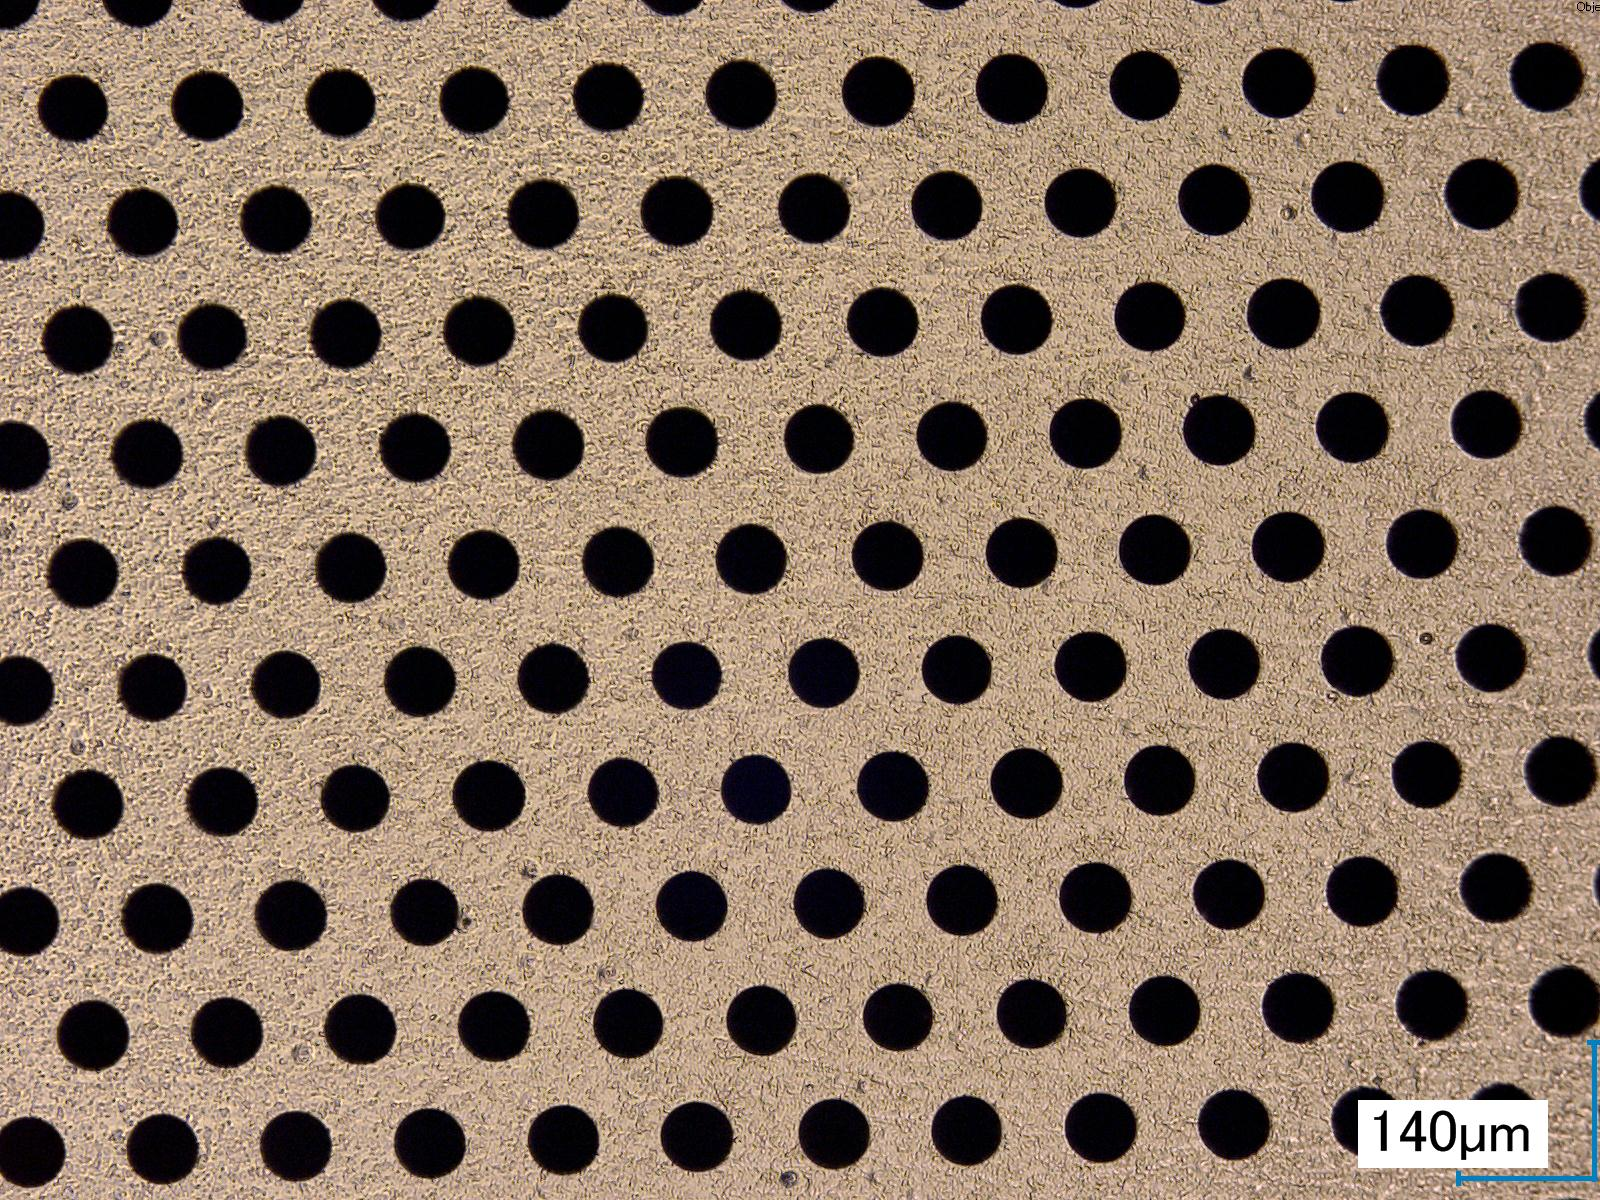
\includegraphics[scale=0.15]{Topside_UpperLeft.jpg}
		\caption{Draufsicht auf Folienausschnitt aufgenommen mit einem Digitalmikroskop Modell VHX-200 \cite{MikroskopReinraum}, ausgezeichnet ist der ein Maßstab von $140 \si{\mu m}$}
		\label{fig:Draufsicht}
	\end{figure}

	\begin{figure}[h]
		\centering
		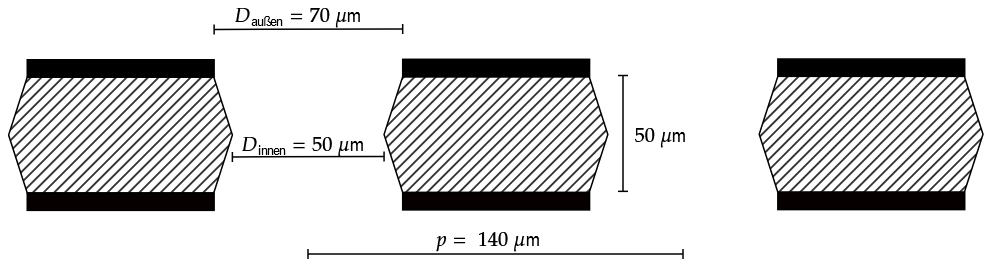
\includegraphics[scale=0.5]{Querschnitt GEM.png}
		\caption{Querschnitt der Folie}
		\label{fig:Querschnitt}
	\end{figure}
		
		
\noindent Der Vorteil dieser Geometrie ist hierbei ersichtlich. Mit moderatem Spannungen sind hohe Verstärkungen erreichtbar, sodass ein effizienter Betrieb der GEM möglich ist. Sollten die Felder dennoch zu hoch gewählt werden, kann der Multiplikationsprozess außer Kontrolle geraten und zu einer Gasentladung in der Verstärkerfolie führen. Da die Ausleseelektronik aber nunmehr von der Verstärkerstufe elektronisch getrennt ist, sinkt die Wahrscheinlichkeit, dass die Entladung bis zur Auslese propagiert und diese beschädigt. Der Schaden begrenzt sich ggf. auf die Folie.\\
Ferner sind die einzelnen Verstärkungsvolumina nun von den GEM-Elektroden begrenzt, die Feldlinien (Abbildung) verlaufen zwischen der Ober- und Unterseite. Da die Ionen den Feldlinien folgen, ist die Strecke, die sie im Vergleich zu ordinären Proportionalkammern zurücklegen müssen, um zu rekombinieren deutlich kleiner, sodass Verzerrungen durch Ladungswolken deutlich später auftreten. Dies ermöglicht prinzipiell höhere Verstärkungen und höhere Ereignisraten. 		
\\
Da es sich bei den einzelnen GEM-Löchern im Wesentlichen um Proportionalkammern handelt, gelten die in Abschnitt \ref{sec:IonisationsundProportionalkammern} diskutierten Grenzen für jedes der Löcher individuell.
			



\section{Multi-GEM-Strukturen}
	Neben den bisher erörterten Vorteilen wird das volle Potenzial von GEM-Stufen erst dann ausgeschöpft, wenn mehrere Stufen hintereinander geschaltet werden. Auf diese Weise können die Elektronen, die aus einer ersten Verstärkungsstufe hervorgehen, an eine zweite Stufe übergeben werden, um dort weitere Multiplikationsschritte zu durchlaufen. Dies ermöglicht das Erreichen hoher Verstärkungen mit geringerem Aufwand und reduziert somit die Häufigkeit von Gasentladungen. \\
	Die Übergabe zwischen den Verstärkungstufen erfolgt über Driftkammern. So werden Gasentladungen zwischen den Folien verhindert, und Diffusionseffekte sorgen dafür, dass die Elektronen aus einer Verstärkungsstufe nicht nur in ein einzelnes GEM-Loch der nachfolgenden Stufe gelangen, sondern in mehrere. Dies erlaubt es, das Raether-Limit für Proportionalkammern effektiv zu umgehen und höhere Verstärkungen zu erzielen, ohne das Risiko von Gasentladungen signifikant zu erhöhen. Eine solche Konfiguration wird als Multi-GEM-Detektor bezeichnet.\\
	\\
	 In Abbildung \ref{fig:Konzeptskizze GEM Aufbau} wird der schematische Aufbau eines Triple-GEM Detektors gezeigt. Hierbei ahmt die Abbildung die tatsächliche Struktur des verwendeten Setups nach, statt auf die konzeptionelle Funktionsweise zu setzen. Diese Anordnung der Folien ist Resultat zahlreicher Optimierungsversuche. In diesem Kontext hat sich gezeigt, dass der Störeinfluss durch die Ionen noch effektiver reduziert werden kann, wenn die Folien um $90^{\circ}$ gegeneinander rotiert werden. Dies limitiert die Ionen auf den Bereich zwischen zwei GEM-Folien und verhindert so erhebliche Störungen durch die Propoagation der Ionen durch den Detektor.
	
	\begin{figure}[h]
		\centering
		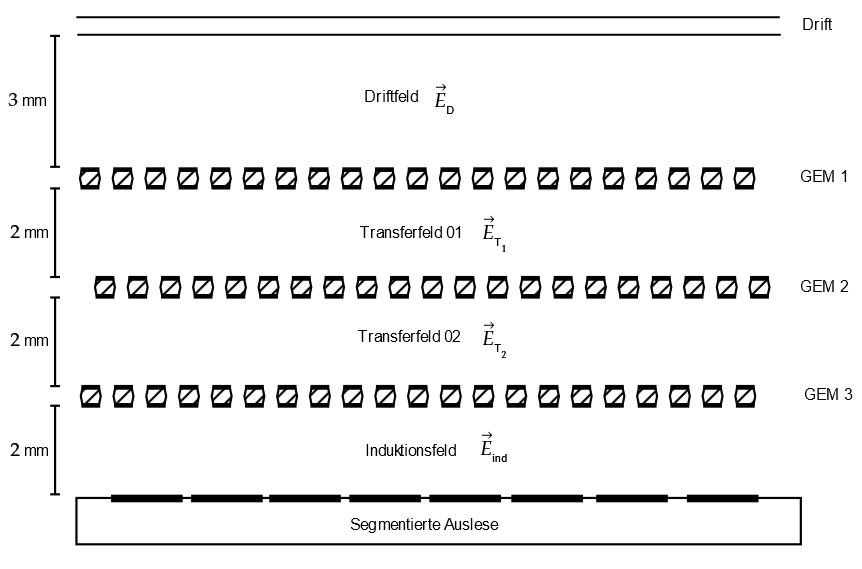
\includegraphics[scale=0.5]{Querschnitt Detektor.png}
		\caption{Querschnitt eines Triple-GEM Detektors mit segmentierter Ausleseelektronik. Die Abstände der einzelnen Stufen zueinander sind auf das verwendete Setup angepasst, zusätzlich wurde die Nomenklatur der Felder angepasst (modifiziert nach \cite{Sauli_Übersicht})}
		\label{fig:Konzeptskizze GEM Aufbau}
	\end{figure}
	
	
	\newpage

\section{Effektive Gain und Transfereffizienzen}
In einem Idealen System würden alle Elektronen, die bei der Verstärkung erzeugt werden auch in die nächste Verstärkerstufe und so zur Ausleseelektronik gelangen. In der Praxis ergeben sich im Wesentlichen drei Wege, über die Elektronen für die anderen Stufen verloren gehen können:
\begin{enumerate}
	\item Wechselwirkung mit der oberen Kupferplatte: Die Elektronen werden von dem GEM-Feld im Allgemeinen in das Loch gesaugt, es gibt jedoch einen Teil der Elektronen, die nicht eingesaugt werden, sondern von der Kupferplatte abgefangen werden. Diese Elektronen stehen offenbar nicht mehr für die Verstärkung zur Verfügung
	\item Verluste durch Polyamid-Interaktion: Elektronen, die in die Verstärkerstufe aufgenommen wurden, können von der Berandung der Löcher aufgenommen werden und stehen so nicht mehr zur Verfügung
	\item Wechselwirkungen mit der unteren Kupferplatte: Die Elektronen, die aus der Verstärkerstufe extrahiert werden, können bei der Extrahktion durch das GEM-Feld auf die untere Platte beschleunigt werden. Diese können dann offenbar nicht mehr weiterverwendet werden. 
\end{enumerate}
Physikalisch steht dahinter die Intuition, ob die Felder in einer Art zusammenwirken, die die Übergabe der Elektronen der Drift- und Transferfelder an GEM-Stufen begünstigen oder erschweren. Zu diesem Zweck definieren wir die Transfereffizienzen:
\begin{equation*}
	\epsilon_{\text{coll}}=\frac{N_{\text{gesammelt}}}{N_{\text{ein}}} \quad \epsilon_{\text{extr}}=\frac{N_{\text{extr}}}{N_{\text{extr}}+N_{\text{verl}}}
\end{equation*}
Hierbei bezeichnet die Kollekttionseffizienz $\epsilon_{\text{coll}}$ die Zahl der aus einer Stufe eingesammelten Ladungen normiert auf die Zahl der gesamt-einfallenden Ladungen und die Extraktionseffizienz $\epsilon_{\text{extr}}$ das Verhältnis der extrahierten Ladung normiert auf die Gesamtladung, die sich aus der extrahierten und der verlorenen Ladung zusammensetzt. Die Transfereffizienten verändern dabei offenbar die Verstärkung. Unter der Annahme, dass eine GEM-Stufe eine Absolute Verstärkung $G_{\textbf{abs}}$ hat, ergibt sich unter Verwendung der Transfereffizienzen folgender Zusammenhang:
\begin{equation}
	G_{\text{eff}}= \epsilon_{\textbf{coll}} \epsilon_{\text{extr}} G_{\text{abs}}
\end{equation}
Die effektive Verstärkung ist hierbei offenbar die Messbare Quantität und ist im Allgemeinen kleiner als die Absolute Verstärkung. Die Transfereffizienzen waren in der Vergangenheit bereits Thema von unterschiedlichen Verständnis und Optimierungsprozessen. In diesem Zusammenhang konnte gezeigt werden, dass die Transfereffizienzen vom Verhältnis der angrenzenden Felder abhängig ist. Insbesondere sind die Kollektionseffizienzen also abhängig von dem GEM-Feld und dem Feld, dass die Teilchen übergibt; die Extraktionskoeffizienten sind abhängig vom den GEM-Feldern und dem Feld, dass die Elektronen extrahiert.
	\newpage
	\chapter{Optimierung der Verstärkung eines Triple GEM Detektors}

	\section{Aufbau des Detektors}
		\subsection{Detektorkonfiguration}
	Die systematische Erfassung von Verstärkung und Energieauflösung erfordert eine Detektoranordnung, die die flexible Variation der Felder ermöglicht und vergleichsweise einfach zu unterhalten ist. Zu diesem Zwecke wird die Konfiguration aus Abbildung \ref{fig:Konzeptskizze GEM Aufbau} in einem eigens für solche Zwecke konzipierten Detektor gebaut \cite{DetektorPrototyp}. \\
	\\
	 Hierzu werden die GEM-Folien auf Rahmen gespannt, die es ermöglichen die Folien in eine dafür vorgesehene Halterung einzusetzen ( siehe Abbildung (\textcolor{blue}{Hier CAD-Zeichnung des Detektors einfügen, weil Software unbekannt nehme ich vielleicht die aus Ottnad,2020?})), der Abstand der einzelnen Folien und Platten kann variabel über Abstandsbolzen eingestellt werden. Die Rahmenanordung wird dann in dem Aluminiumgehäuse fixiert. Das Alumniniumgehäuse bietet dabei Anschlüsse für die Hochspannungskabel zum Betrieb des Detektors, sowie Anschlüsse zur Auslese der Messereignisse und Anschlüsse für Gaszu- und Abfluss. Die Strahlung kann durch dafür vorgesehene Fenster eingestrahlt werden, die auf dem Aluminumverdeck und an der Seite sind. Für den Fall der Einstrahlung von oben wurde die Driftfeldanode in zwei Anoden aufgeteilt, da so Elektronen-Ionen-Paare, die über der Driftkammer entstehen von der oberen Platte abgefangen werden können und so keine Schwankungen im Driftfeld zulässt. Auf diese Weise wird der Detektor sicherer gegen Störeinflüsse geschützt.

		\subsection{Auslese- und Betriebselektronik}
		In diesem Absatz sollen die Grundlagen der verwendeten Elektronik beschrieben und begründet werden. In Abbildung \textcolor{blue}{Blockschaltbild von Betriebs und Ausleseelektronik}. ist das Konzeptionelle Blockschaltbild zu sehen, mit dem die Messungen stattfinden. Die GEM-Folien werden über einen Hochspannungsgenerator des Modells betrieben, wobei ein Pikoamperemeter des Typs \textcolor{red}{Zagreb-Pikoampermeter-Ident} davorgeschaltet wird. Dies ermöglicht die Detektion von Gasentladungen, durch die kurzweilige aber vergleichsweise große Ströme entstehen können, wobei dann Schritte ergriffen werden können, um die Detektoranordnung vor großflächigeren Schäden zu schützen. Die Spannungen sind über eine zentralisierte Slow-Control steuerbar und können anwendungsbedingt auf eine Genauigkeit von einem Volt \textcolor{red}{Verifikation} eingestellt werden. \textcolor{red}{gehe auf die Süezifikationen der Schaltung ein, siehe Ottnad Arbeit} \\
		\\
		Die Ausleseanordnung besteht aus einem Vorverstärker des Modells \textcolor{red}{Modelltyp und Verstärkung} und einem Impulsformenden Verstärker des Modells \textcolor{red}{Modelltyp}. Hier sind die Verstärkung und die Signalformzeit aus gegebenen Einstellungen wählbar. Das geformte und Verstärkte Signal wird dann auf einen Vielkanalzähler gegeben, welcher die einkommenden Signale auf einzelne Bins je nach Amplitude verteilt. Das resultierende MCA-Spektrum kann dann entweder durch die Slow-Control oder ein dafür vom Hersteller vorgesehenes Programm aufgenommen werden.\\
		Alternativ kann die Auslese auch direkt an einen anderen Kanal des Pikoamperemeters angeschlossen werden, um den in der Messelektonik induzierten Strom zu bestimmen. Es ergibt sich ein Blockschaltbild wie in Abbildung \textcolor{red}{Blockschaltbild II}  
		
		\subsection{Gasqualitätssicherung und Druck-Temperatur-Überwachung}
		Neben einer starken Feldabhängigkeit ist die effektive Verstärkung in einem GEM-Detektor auch abhängig von dem Druck und der Temperatur des aktiven Mediums. Da das System nicht komplett isolierbar ist, müssen Druck und Temperaturschwankungen entsprechend überwacht und deren Einfluss aus den Messergebnissen rausgerechnet werden. Insbesondere sind Unreinheiten im Gas nicht gewünscht, sodass auch die Verunreinigungen des Gases überwacht werden müssen.\\
		\\
		Zum Überwachen der Druck- und Temperaturschwankungen wird dazu ein Laborlogger verwendet. Hierbei wird ein Sensor der Klasse MS5611 verwendet, der Prinzipiell im Stande dazu ist Druck, Temperatur und Luftfeuchte zu messen \cite{LoggerSensor}. Die Genauigkeit der Druckmessung liegt dabei  bei $\pm 1.5 \si{mbar}$  ; die Genauigkeit der Temperaturmessung liegt bei $\pm 0.8 \si{^\circ C}$. Der Sensor wird über einen Microcontroller des Typs \textcolor{red}{Typ Microcontroller} ausgelesen und die Daten werden an eine Datenbank übergeben \cite{Hauer}.\\
		Die Reinheit des Gases wird durch einen Vielgasanalysator des Modells \textcolor{red}{Rapidoxmodell} überwacht. Hierbei werden Sauerstoff- und Wassergehalt gemessen. 
		

	\section{Messmethodik}
		\subsection{Über die Eignung von $\ce{^{55}}$Fe-Isotopen}\label{sec:Fe55}
			Die Untersuchung der Effekte der einzelnen Felder eines Triple-GEM-Detektors auf seine Energieauflösung und Verstärkung erfordert eine fundierte Kenntnis der zur Messung verwendeten Strahlung. Eine geeignete Strahlenquelle muss daher einige Anforderungen erfüllen, um den Optimierungsprozess zu ermöglichen. Die Eignung einer  $\ce{^55Fe}$ Quelle kann dabei wie folgt begründet werden:\\
			\\
			Das Isotop $\ce{^55Fe}$ zerfällt durch Elektronen-Einfang zu Mangan, welches durch Emission von Röntgenstrahlung in seinen Grundzustand übergeht, das resultierende Mangan-Isotop $\ce{^55 Mn}$ ist stabil. Mit einer Halbwertszeit von 2,75 Jahren \cite{Half_Life_FE55} gewährleistet die Quelle während des gesamten Optimierungsprozesses eine konstante Strahlleistung und so einen stabilen Energiepegel. Insbesondere sind Verzerrungen durch Sekundärzerfälle ausgeschlossen.\\
			Das Spektrum wird hauptsächlich von den $K_{\alpha}$- und $K_{\beta}$-Linien dominiert, was sicherstellt, dass die gesamte Energie im System deponiert wird (siehe Kapitel \ref{chap:Photonen}). Dadurch werden statistische Unsicherheiten in der Energiedeposition und damit verbundene Einflüsse auf die Energieauflösung minimiert. Eine Sammlung der relevanten Eisenlinien findet sich in Tabelle \ref{tab:Eisenlinien}.
			
			\begin{table}[h!]
				\centering
				\begin{tabular}{|l|c|c|}
					\hline
					\textbf{Linie} & \textbf{Energie / keV} & \textbf{Rel. Intensität} \\ \hline
					K\textsubscript{$\alpha$}-Photo 1    & 5,755         & 0,540           \\ \hline
					K\textsubscript{$\alpha$}-Photo 2    & 5,716         & 0,117           \\ \hline
					K\textsubscript{$\alpha$}-Photo 3    & 5,815         & 0,078           \\ \hline
					\textbf{K\textsubscript{$\alpha$}-Photo}  & 5,755         & 0,777           \\ \hline
					\textbf{K\textsubscript{$\alpha$}-Escape} & 2,892         & 0,121           \\ \hline
					K\textsubscript{$\beta$}-Photo 1     & 6,351         & 0,061           \\ \hline
					K\textsubscript{$\beta$}-Photo 2     & 6,312         & 0,013           \\ \hline
					K\textsubscript{$\beta$}-Photo 3     & 6,411         & 0,009           \\ \hline
					\textbf{K\textsubscript{$\beta$}-Photo}  & 6,351         & 0,088           \\ \hline
					\textbf{K\textsubscript{$\beta$}-Escape} & 3,488         & 0,014           \\ \hline
				\end{tabular}
				\caption{relevante Linien des Eisenspektrums einer $\ce{^55 Fe}$-Quelle in Argon, entnommen aus \cite{ottnad}. Hervorgehoben sind die Linien, die das Signal dominieren}
				\label{tab:Eisenlinien}
			\end{table}
			
			
			\noindent Die im Optimalfall erreichbare Energieauflösung überschreitet die Energieabstände der einzelnen $K$ Linien. Diese Aussage trifft sowohl für den Photopeak, als auch für den Escape-Peak zu, sodass diese offenbar nicht eindeutig auflösbar sind. Entsprechend müssen nur wesentliche Linien berücksichtigt werden
			
			
			
			 Die Bestimmung der Detektorparameter stützt sich auf die Bestimmung der Parameter des Photopeaks, es wird demnach das Spektrum angepasst, das aufgrund der Nähe der Linien vollumfänglich durch folgende Funktion beschrieben werden kann \cite{Hauer}. für die folgende Diskussion, sollen die einzelnen Signalteile entsprechend ihrer Bedeutung diskutiert werden.
			 

			\begin{enumerate}
				\item \textbf{Photopeak} Der Photopeak setzt sich aus den Photopeaks für $\text{K}_{\alpha}$- und $\text{K}_{\beta}$-Linie zusammen. Um die Zahl der freien Parameter des Modells zu verkleinern nutzen wir, dass die relativen Intensitäten zu einem Skalierungsfaktor von $8,83$ führen:
				\begin{equation*}
					{ I_{\text{ph}}= A_{{\alpha}} \qty(\exp(\frac{1}{2}\qty(\frac{x-\mu_{{\alpha}}}{\sigma_{\alpha}})^{2})+ \frac{1}{8,8}\exp(\frac{1}{2}\qty(\frac{x-\mu_{{\beta}}}{\sigma_{{\beta}}})^{2}))}
				\end{equation*}
				
				\item \textbf{Escapepeak} Der Escape-Peak wird ein analoger Fit durchgeführt:
				\begin{equation*}
					{    I_{\text{esc}}= A_{{\alpha}}^{\text{Esc}} \qty(\exp(\frac{1}{2}\qty(\frac{x-\mu_{{\alpha}}^{\text{Esc}}}{\sigma_{\alpha}^{\text{Esc}}})^{2})+ \frac{1}{8,8}\exp(\frac{1}{2}\qty(\frac{x-\mu_{{\beta}}^{\text{Esc}}}{\sigma_{{\beta}}^{\text{Esc}}})^{2}))}
				\end{equation*}
				
				\item \textbf{Exponentieller Offset} Es gibt einen Beitrag durch elektronisches Rauschen und durch niederenergetische Fluoreszenz.  Um für diese Effekte zu accounten, schieben wir einen Offset der folgenden Form ein:
				\begin{equation*}
					I_{\text{Off}}= A_{\text{off}} e^{-\frac{x}{c_{\text{char}}}}
				\end{equation*}
				
				\item \textbf{Errorfunction} Auch hier zählen wir das Elektronische Rauschen zu und berücksichtigen, dass das Rauschen am MCA irgendwann nicht mehr zu den Spektren beitragen kann, da kein Signal vorliegt, dass zu einer Signalamplitude in der jeweiligen Range sorgt (quasi Diskriminatorrauschen).
				\begin{equation*}
					I_{\text{erf}}= A_{\text{erf}} \qty(\erf\qty(\frac{x-\mu_{\alpha}}{\sigma_{\alpha}})-1)
				\end{equation*}
			\end{enumerate}
			
			
			
		\subsection{Experimentelle Bestimmung der Verstärkung} \label{sec:Verstärkungsbestimmung}
		Die Bestimmung der Verstärkung wird im folgenden auf zwei Unterschiedliche Wege durchgeführt. Die Methoden sind hierbei auf ihren jeweiligen Zweck, nämlich der quantitativeren oder qualttativeren Verstärkungsbestimmung zugeschnitten.\\
		Die qualtitative Bestimmung der Verstärkung nutzt aus, dass der MCA die Zuordnung zu seinen Bins proportional zur Amplitude des eintreffenden Signals durchführt. Nimmt man für die einzelnen Feldeinstellungen dann ein Spektrum auf, und passt eine Funktion nach Gleichung [REFERENZ] an, dann kann der Peakschwerpunkt des Photopeaks als Funktion der Felder als Proxy für die Verstärkung gewählt werden. Wandert der Schwerpunkt zu höheren Bins, sind die Signalampltiduden offenbar größer und die Signale wurden vorher stärker Verstärkt. Eine solche Methode ist offenbar nur dann sinntragend, wenn es eine Referenz gibt, zu der die Verstärkung relativ untersucht werden kann es handelt sich daher um eine qualitiative Messmethode.\\
		\\
		Quantitativ kann die Verstärkung aus einer Messung des Spektrums und einer Messung des an der Ausleseelektronik induzierten Stromes bestimmt werden. Dazu kann die Auslese des Detektors mit einem Picoamperemeter (MODELL) verbunden werden, sodass die Influenzierten Ströme gemessen werden. In einer darauffolgenden Messung muss dann in derselben Einstellung ein Spektrum gemessen werden; eine parallele Messung ist nicht möglich, da Rauscherscheinungen, die mit den Bauteilen einhergehen einen sehr erheblichen Störeinfluss implizieren, der die Messung nahezu unbrauchbar macht.\\
		Da die Linien der Eisenquelle [ABSCHNITT] hinreichend bekannt sind, können die Linien für eine Energiekalibrierung des MCA für eine gegebene Detektorkonfiguration durchgeführt werden. Damit wird das mit dem MCA gemessene Spektrum zu einem Energie-Histogramm gegebener Bin-weite. Summiert man die einzelnen Ereigniszahlen, gewichtet mit den Energien des jeweiligen Bins auf, erhält man eine Approximation für die im Detektor deponierte Energie und so, unter Berücksichtigung der mittleren Ionisationsenergie (Tabelle \ref{tab:Ionisationsenergien}) eine Näherung für den primären Ionisationsstrom, sofern man die Messdauer berücksichtigt. Die Verstärkung ergibt sich dann entsprechend über den folgenden Zusammenhang:  
		\begin{equation*}
			G=\frac{I_{\text{Readout}}}{I_{\text{Ion}}}
		\end{equation*}
		Es ist offenbar so, dass die quantitative Messung 
		\newpage
	
	\section{Optimierungsmethodik}
	Um eine Optimierung durchführen zu können, wird zunächst eine Referenzmessung durchgeführt. Die aus \cite{ottnad} folgenden Feldeinstellungen (siehe Tabelle \textcolor{red}{Feldertabelle}) werden getestet, um eine für das verwendete Detektorsetup spezifische Vergleichsgröße bestimmen zu können. Diese Referenzgrößen bieten dann die Eckdaten, die die Grundlage des Optimierungsprozesses darstellen.\\
	Der eigentlichen Optimierung wird dann eine Reihe von Analysemessungen vorgeschaltet. Das Ziel dieser Analyse ist es herauszufinden, ob es ein Operationsoptimum im Hinblick auf die Transfereffizienzen gibt, welches es erlaubt die Zahl der für die Optimierung günstigen Detektorkonfigurationen zu reduzieren. Sofern Bedarf besteht, können Einstellungen größerer Verstärkung als Interimskonfigurationen verwendet werden, sofern sie stabile und effiziente Messungen erlauben. Die Analysemessungen sind demnach als iterativer Prozess durchzuführen.\\
	\\
	Um aus den Ergebnissen nun auf potentiell interessante Feldkonfigurationen zu schließen können die Ergebnisse der Analyse verwendet werden, um die Gesamtheit aller Felder aufeinander abzustimmen. Dieses Verfahren soll dabei sicherstellen, dass sowohl die Energieauflösung, als auch die effektive Verstärkung vergleichbar mit den Referenzparametern sind 
	
	\section{Referenzbestimmung}
		\subsection{Methode}
		Über die zentrale Steuerungeinheit lassen sich Feldkonfigurationen vergleichsweise einfach eintragen. In einem ersten Schritt werden daher die Feldeinstellungen aus \cite{ottnad} untersucht, um sicherzustellen, dass die simulierten Ergebnisse mit den Ergebnissen des COMPASS-Experimentes übereinstimmen. In diesem Zusammenhang lassen sich dann die Vergleichsparameter für die Energieauflösung und die effektive Gain bestimmen. Die Einstellungen der Feldkonfigurationen sind in Tabelle \ref{tab:RefKonfig}
		\begin{table}[h!]
			\centering
			\begin{tabular}{|c|c|c|}
				\hline
				&COMPASS & Simulation \\
				\hline
				$E_{\text{D}}\ / \ \ \si{V/cm}$ & 2490 & 2490\\
				\hline
				$U_{\text{GEM}\ 1}/\ \ V$ & 410 & 406  \\
				\hline
				$E_{\text{TF}1} /\ \ \si{V/cm}$ & 3730 & 1753 \\
				\hline
				$U_{\text{GEM}\ 2}/\ \ V$ & 374 & 367  \\
				\hline
				$E_{\text{TF}2} /\ \ \si{V/cm}$ & 3730 & 1578 \\
				\hline
				$U_{\text{GEM}\ 3}/\ \ V$ & 328 & 322  \\
				\hline
				$E_{\text{ind}}/\ \ \si{V/cm}$ & 3730 & 3730  \\
				\hline
			\end{tabular}
			\caption{Sammlung der Detektorfeldkonfigurationen basierend auf den Einstellungen des COMPASS-Experiment und der Ergebnisse der Simulationsergebnisse. Die Originaleinstellungen aus \cite{ottnad} wurden auf die verwendete Gasmischung reskaliert}
			\label{tab:RefKonfig}
		\end{table}
		
		
		
		\noindent Um sicherzustellen, dass die Vergleichsmessungen für beide Einstellungen vergleichbar sind, muss zunächst eine Verstärkerkonfiguration bestimmt werden, die beide Konfigurationen auf dem MCA hinreichend gut auflöst, um sicherzustellen, dass der Anpassungsprozess für beide Spektren funktioniert. Die Messung der Verstärkung wird dann nach dem in Abschnitt \ref{sec:Verstärkungsbestimmung} Verfahren durchgeführt.
		
		\subsection{Ergebnisse}
		
	
	
	
	\newpage
	\section{Parameterscans für die einzelnen Felder}
		\subsection{Untersuchung der Wirkung der Felder auf die Transfereffizienzen}
		
		\subsection{Bestimmung der Auswahlintervalle}
	
	
	\newpage
	\section{Konstruktion und Überprüfung interessanter Detektorkonfigurationen}


\newpage
\chapter{Optimierung der Energieauflösung eines Triple-GEM-Detektors}
	\section{Messmethodik}
	
	\section{Optimierungsmethodik}
	
	\section{Parameterscans für die einzelnen Felder}
	
	\section{Konstruktion und Überprüfung interessanter Detektorkonfigurationen}
	
	
\chapter{Bestimmung des Operations-Optimums}
	\section{Konstruktion von Feldkonfigurationen unter Berücksichtigung von Auflösung und Verstärkung}
	
	\section{Experimentelle Analyse der Konstruierten Konfigurationen}
	
\chapter{Zusammenfassung und Ausblick}
	\section{Zusammenfassung}
	
	\section{Ausblick: Optimierung auf Orts- und Zeitauflösung}		

	\newpage
	\appendix % Appendix: Quality Assurance Messungen
	\printbibliography
	
\end{document}